\section{Results}
\label{sec:results}

\subsection{Where the Gain Comes From}
\label{sec:decomp}

The modernized tracker (YOLOv8m + OSNet) raises mean HOTA from \baselineHOTA{} to \modernHOTA{}
($+\deltaHOTA$) and exceeds the baseline on every one of the six videos (\cref{tab:fullpipeline}).
Decomposing the gain on the combined MOT16 split (\cref{tab:decomp}) shows it is detection-dominated:
the detection term improves by $\detaGain$ HOTA points while the association term improves by only
$\assaGain$. MOTA barely moves ($\baselineMOTA \rightarrow \modernMOTA$), as expected for a
detection-recall-dominated metric, which is precisely why we report HOTA.

\begin{table*}[t]
\centering
\caption{Per-video HOTA: unmodified baseline vs.\ the modernized pipeline.}
\label{tab:fullpipeline}
\small
\begin{tabular}{lccccccc}
\toprule
\textbf{Configuration} & TUD-Campus & TUD-Stadt. & KITTI-17 & PETS09 & MOT16-09 & MOT16-11 & \textbf{Mean} \\
\midrule
Baseline (provided det.\ + mars) & 39.86 & 36.75 & 43.41 & 44.84 & 36.24 & 39.95 & 40.17 \\
\textbf{Modern (YOLOv8m + OSNet)} & \textbf{46.98} & \textbf{59.62} & \textbf{48.75} & \textbf{60.28} & \textbf{48.57} & \textbf{51.07} & \textbf{52.54} \\
\bottomrule
\end{tabular}
\end{table*}

\begin{table}[t]
\centering
\caption{Decomposition on the combined MOT16 split.}
\label{tab:decomp}
\small
\begin{tabular}{lccccc}
\toprule
 & HOTA & MOTA & IDF1 & DetA & AssA \\
\midrule
Baseline & 38.65 & 46.34 & 50.65 & 37.85 & 39.52 \\
Modern   & 47.68 & 46.75 & 52.18 & 50.15 & 45.77 \\
$\Delta$ & +9.03 & +0.41 & +1.53 & \textbf{+12.30} & +6.25 \\
\bottomrule
\end{tabular}
\end{table}

The same conclusion holds from the association side. Replacing the detector with a ground-truth-box
oracle isolates association quality: a dedicated OSNet reaches \osnetGT{} HOTA, but a generic,
non-re-ID-trained ImageNet backbone reaches \timmGT{} -- a gap of under one HOTA point
(OSNet-AIN \osnetainGT{} is intermediate). Once detection is held perfect, association quality is
nearly detector-bound and the choice of appearance model is almost free. The gain from
modernization therefore lives overwhelmingly in the detector.

This makes the \emph{quality} of the detection stream, not its raw quantity, the operative variable.
\cref{tab:detector} reports YOLOv8m precision, recall, and F1 against ground truth at
IoU~$\geq 0.5$. Recall is uniformly high (mean $0.831$), but precision is strongly clip-dependent:
high on clean sequences (TUD-Stadtmitte $0.907$, PETS09 $0.858$) and low on the dense,
low-resolution clips (TUD-Campus $0.505$, KITTI-17 $0.514$), where the detector emits roughly as many
false positives as true ones. This per-clip precision is the quantity that, below, predicts whether
adding detections helps or hurts.

\begin{table}[t]
\centering
\caption{YOLOv8m detection quality vs.\ ground truth (IoU~$\geq 0.5$, conf~0.25).}
\label{tab:detector}
\small
\begin{tabular}{lccc}
\toprule
\textbf{Sequence} & Precision & Recall & F1 \\
\midrule
TUD-Campus     & 0.505 & 0.869 & 0.639 \\
TUD-Stadtmitte & 0.907 & 0.863 & 0.884 \\
KITTI-17       & 0.514 & 0.867 & 0.645 \\
PETS09-S2L1    & 0.858 & 0.950 & 0.901 \\
MOT16-09       & 0.650 & 0.743 & 0.693 \\
MOT16-11       & 0.663 & 0.694 & 0.678 \\
\midrule
\textbf{Mean}  & \textbf{0.683} & \textbf{0.831} & \textbf{0.740} \\
\bottomrule
\end{tabular}
\end{table}

\subsection{When More Detections Hurt}
\label{sec:hurt}

We sweep the detector confidence threshold per video over $\{0.15, 0.25, 0.35, 0.45\}$, holding
everything else fixed. Lowering the threshold raises recall and lowers precision; the question is what
this does to HOTA. \cref{fig:hota_vs_conf} shows the response is not monotone in a fixed direction
across clips: on the dense, low-precision clips HOTA \emph{increases} as the threshold rises (i.e.\
adding low-confidence detections \emph{hurts}), whereas on the clean clips it is flat or mildly
decreasing. On \nHurt{} of the \nVideos{} videos, raising the precision gate improves HOTA.

The sign of recall's effect is predicted by per-clip detector precision. \cref{fig:money} plots, for
each video, the change in HOTA from the lowest to the highest confidence threshold against the clip's
detector precision (\cref{tab:detector}); the two are correlated (Pearson $r = \corrPearson$): the
lower a clip's detector precision, the more it benefits from a higher confidence gate. An orthogonal
recall lever confirms the effect is a property of recall itself rather than of one knob. On the two
dense clips we instead sweep the detector input resolution (\cref{fig:imgsz}); on TUD-Campus, raising
the input size drives HOTA monotonically \emph{down}
($\imgszLow \rightarrow \imgszMid \rightarrow \imgszHigh$). More pixels recover more small instances,
and the extra, lower-quality detections degrade tracking exactly as lowering the confidence threshold
does.

\begin{figure}[t]
\centering
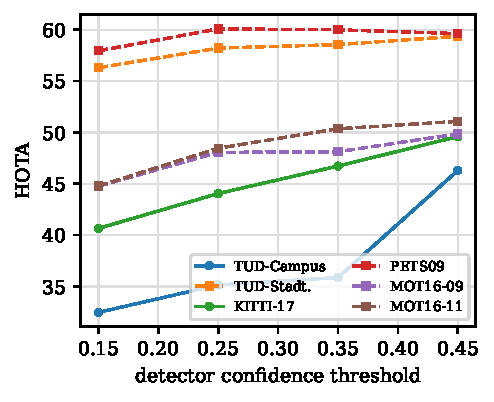
\includegraphics[width=\columnwidth]{figures/fig_hota_vs_conf.pdf}
\caption{HOTA vs.\ detector confidence threshold per video. Solid lines are the dense, low-precision
clips; on them HOTA rises as weak detections are filtered out.}
\label{fig:hota_vs_conf}
\end{figure}

\begin{figure}[t]
\centering
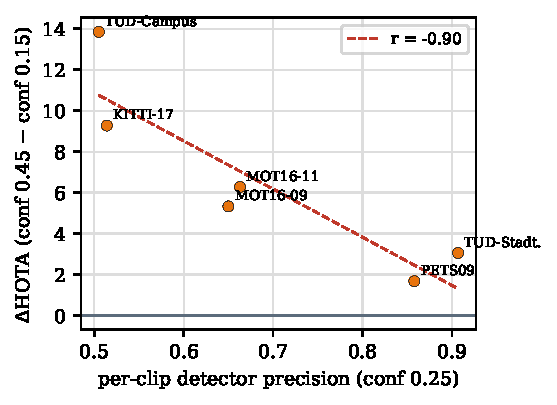
\includegraphics[width=\columnwidth]{figures/fig_money_plot.pdf}
\caption{The sign and size of recall's effect on HOTA (here, HOTA at conf~0.45 minus conf~0.15) track
per-clip detector precision: low-precision clips gain most from a higher confidence gate.}
\label{fig:money}
\end{figure}

\begin{figure}[t]
\centering
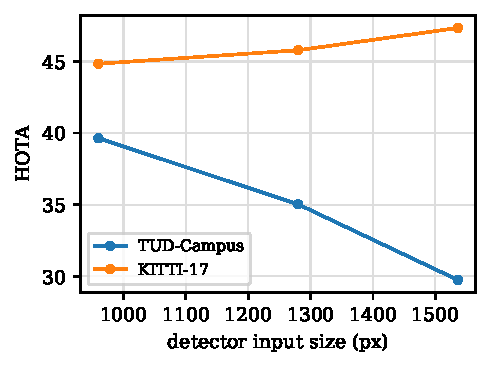
\includegraphics[width=\columnwidth]{figures/fig_imgsz_dense.pdf}
\caption{Input-size sweep on the two dense clips. Raising resolution (an orthogonal recall lever)
lowers HOTA, mirroring the confidence sweep.}
\label{fig:imgsz}
\end{figure}

\subsection{The Dropped Gate: a Restoration Ablation}
\label{sec:ablation}

To attribute the regression to the dropped gating contract rather than to the detector itself, we
restore the original DeepSORT gate -- $\text{min\_confidence}=0.3$ with NMS at overlap~$0.7$ -- on top
of the otherwise unchanged modern pipeline (\cref{fig:ablation}). Restoring the gate recovers HOTA on
the dense clips (mean $\ablationRecover$ HOTA on TUD-Campus and KITTI-17) while leaving the clean
clips essentially unchanged. Because the restored gate is the same confidence-plus-NMS filter the
original method applied, re-enabled by configuration alone, the recovered HOTA is causally
attributable to the gate.

\begin{figure}[t]
\centering
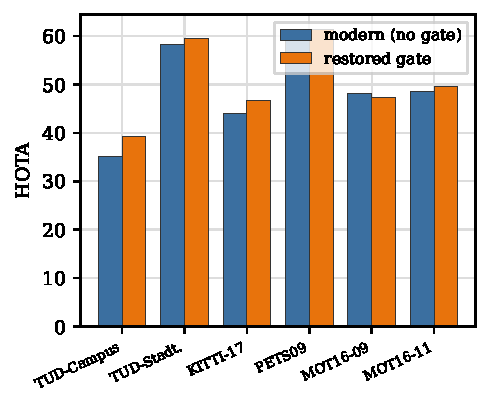
\includegraphics[width=\columnwidth]{figures/fig_ablation.pdf}
\caption{Gating-restoration ablation: per-video HOTA with the modern (ungated) pipeline vs.\ the
restored original confidence + NMS gate.}
\label{fig:ablation}
\end{figure}

\subsection{A Per-Clip Precision-Gating Guideline}
\label{sec:tuning}

The practical consequence is a simple per-clip policy: choose the detector confidence threshold from
the clip's precision regime rather than a single global default. Applied to the worst sequence,
raising the TUD-Campus threshold to $0.45$ moves it from a $\tudUntuned$ HOTA deficit (the global
default loses to the baseline there) to $+\tudGain$ over baseline, and the change is confined to that
sequence's preset, leaving the other five untouched. This single per-video override is what lifts the
modernized tracker to a win on all six videos in \cref{tab:fullpipeline}, at a mean real-time
throughput of \fpsRealtime{}~FPS.
